\documentclass[conference]{IEEEtran}
% ============================================================================
% NDSS 2027 submission (double-blind, anonymized).
% Foundations of interpretability-based trust in ML-based intrusion detection.
% All numbers trace to code/results/*.csv via claims.json.
% ============================================================================
\usepackage{amsmath,amssymb}
\usepackage{graphicx}
\usepackage{booktabs}
\usepackage{multirow}
\usepackage{url}
\usepackage[hidelinks]{hyperref}
\usepackage{amsthm}
\graphicspath{{figs/}}
\newtheorem{definition}{Definition}
\newtheorem{property}{Property}
\newtheorem{claim}{Claim}

\begin{document}
\title{When Is an Explanation Trustworthy?\\
Foundations of Interpretability-Based Trust in\\ Machine-Learning Intrusion Detection}

\author{\IEEEauthorblockN{Anonymous Submission}
\IEEEauthorblockA{Under double-blind review}}

\maketitle

\begin{abstract}
A fast-growing line of work equips machine-learning intrusion detection systems (ML-IDS) with
explanations and argues that the resulting interpretability lets a security analyst
\emph{trust} the detector: verify its reasoning, calibrate confidence, and be accountable for
acting on its alarms. We ask a foundational question this literature leaves implicit: what must
be true of an explanation for such trust to be \emph{well-founded}? We formalize
interpretability-based trust and show it presupposes three properties of the explanation map,
\emph{fidelity} (the interpretable artifact decides as the deployed model does),
\emph{determinacy} (the explanation is fixed by the decision, not by an arbitrary methodological
choice), and \emph{groundedness} (the explanation reflects the task, not the incidental model
instance), each of which we argue is necessary for trust. On three modern network-intrusion
datasets (UNSW-NB15, CICIDS2017, and the 5G-testbed dataset 5G-NIDD), and across five standard
explainers including SHAP and LIME, all three properties fail: interpretable surrogates lose up
to $0.32$ $F_1$; SHAP and LIME, the two most deployed explainers, agree on only about a fifth of
the features they show; and detectors with statistically identical accuracy disagree on nearly
half of their top features. We then ask whether the failure can be exploited by an adversary who
manipulates the explanation while keeping the malicious decision; our attacks on tabular IDS were
inconclusive, an honest negative result that we report and analyze. Finally, we turn the
diagnosis into a defense: a lightweight, per-alarm \emph{reliability gate} predicts, from a
single deployed model, whether an explanation is trustworthy for a given flow, with AUC up to
$0.94$, and we show it is not reducible to an out-of-distribution detector. We distill the study
into threat-aware evaluation criteria that a defensible interpretability-for-trust claim in
security must meet. This reframes an accountability question that operational security
increasingly relies on: interpretability is not, by default, a warrant for trust, but the
conditions under which it would be are checkable, and partly enforceable.
\end{abstract}

% ============================================================================
\section{Introduction}\label{sec:intro}
% ============================================================================
Machine-learning intrusion detection systems (ML-IDS) are opaque, and opacity is a problem in a
setting where a human analyst must decide whether to act on an alarm and is accountable for that
decision. The dominant response is \emph{explainable} intrusion detection: attach to each alarm
an explanation, typically a ranked list of the input features most responsible for it, and argue
that the analyst can now understand, verify, and \emph{trust} the detector. Recent work reports
that explanations raise analyst trust, cut false-positive dismissals, and speed triage, and
surveys frame interpretability as the route to trustworthy and accountable security
AI~\cite{capuano2022}.

This paper asks a question the literature leaves implicit. Trust, in a security setting, is not a
feeling; it is a warrant for action under an adversary. If an analyst escalates or suppresses an
alarm \emph{because} of the explanation, then the explanation is part of the trusted base of the
security operation. So we must ask: \textbf{what must be true of an explanation for the trust
placed in it to be well-founded?} The explainable-IDS literature measures whether explanations
\emph{increase} trust (through user studies, satisfaction scores, triage-time reductions); it
rarely asks whether that trust is \emph{warranted}.

We take up the foundational question and answer it constructively. Our contributions are:

\begin{itemize}
\item We \textbf{formalize interpretability-based trust} for ML-IDS
(Section~\ref{sec:formal}) and derive three properties any explanation must satisfy for the
trust to be sound: \emph{fidelity}, \emph{determinacy}, and \emph{groundedness}. Each is
necessary, so violating any one voids the warrant.
\item We show, on \textbf{three modern NIDS datasets} and \textbf{five standard explainers
(gradient saliency, input$\times$gradient, integrated gradients, SHAP, LIME)}, that all three
properties fail, with multi-seed confidence intervals (Section~\ref{sec:fail}). Notably, SHAP
and LIME agree on only about a fifth of the features they present to the analyst.
\item We ask whether the failure is \textbf{adversarially exploitable}: can an attacker keep a
flow malicious yet make its explanation look benign, so the analyst dismisses a true alarm? Our
tabular attacks were inconclusive; we report this negative result honestly and analyze why
explanation manipulation may not transfer from vision to tabular IDS (Section~\ref{sec:adv}).
\item We turn the diagnosis into a \textbf{defense}: a per-alarm \emph{reliability gate}
(Section~\ref{sec:defense}) that predicts, cheaply and from one deployed model, whether an
explanation is trustworthy for a given flow (AUC up to $0.94$), and which we show is not merely
an out-of-distribution detector.
\item We distill \textbf{threat-aware evaluation criteria} (Section~\ref{sec:criteria}) that a
defensible interpretability-for-trust claim in security must meet.
\end{itemize}

Our aim is neither to argue that ML-IDS should be opaque nor that interpretability is worthless.
It is to show that the inference ``the model is interpretable, therefore its alarms can be
trusted'' is, as currently supported, unsound, to explain what would make it sound, and to give a
first mechanism that recovers part of the warrant. We view this as a foundations-of-security
question: the conditions under which a security control may be relied upon.

% ============================================================================
\section{Motivation and Setting}\label{sec:motiv}
% ============================================================================
Consider a security operations center where an ML-IDS raises an alarm on a network flow and
presents the analyst with the five features most responsible, say a large backward packet
length and a short flow duration. The analyst, trained to read such explanations, judges the
alarm consistent with a known attack and escalates; or, seeing features that look like ordinary
traffic, dismisses it as a false positive. Vendors and recent research encourage exactly this
workflow, and human-factors studies report that analysts act on explanations and trust systems
more when explanations are present.

The workflow embeds an assumption: that the shown features are a reliable account of why the
detector fired. If they are not, the analyst's judgment is untethered from the detector's actual
behavior, and worse, from the ground truth of whether the flow is an attack. Three ways the
account can be untethered motivate our properties. It can reflect a \emph{different model} than
the one deployed (if interpretability is delivered by a surrogate). It can be an artifact of the
\emph{explanation method} rather than the decision (if a different, equally standard method would
have shown different features). And it can be an accident of the \emph{particular trained model}
rather than the task (if an equally accurate retraining would explain differently). We make these
precise next and then measure them.

\textbf{Scope.} We study network intrusion detection on tabular flow features, the setting where
explanations are usually feature attributions over named quantities. We consider standard
attribution explainers rather than prototype- or rule-based methods; extending to those is a
direction our criteria call for. We treat detection itself as given and study the explanation
layer that sits on top of it.

% ============================================================================
\section{Background and Related Work}\label{sec:bg}
% ============================================================================
\textbf{Critiques of ML-IDS evaluation.} A tradition of foundational scrutiny warns that ML
security results often do not mean what they appear to. Sommer and Paxson~\cite{sommer2010}
argued that the closed-world assumptions of ML evaluation break in operational intrusion
detection; Arp et al.~\cite{arp2022} catalogue pervasive experimental pitfalls (spatial and
temporal snooping, base-rate neglect, inappropriate baselines); Axelsson's base-rate
analysis~\cite{axelsson2000} shows why laboratory detection rates mislead at realistic
prevalence. These critiques target \emph{accuracy} claims and their datasets. Ours targets a
newer claim, \emph{interpretability for trust}, that the accuracy critiques do not address.

\textbf{Explainable intrusion detection.} A large recent literature applies attribution methods
(gradient saliency, SHAP, attention) to ML-IDS and argues they enhance analyst trust and
accountability~\cite{capuano2022}. Constructive proposals go further: recent work designs
action-oriented explanations, e.g.\ feasible-action contracts for intrusion
triage~\cite{action2026}. This work builds explanations and measures user-facing trust. We are
orthogonal and adversarial to it: we ask whether the trust so induced is warranted, formalize
the conditions under which it would be, and give a mechanism to flag when it is not.

\textbf{Fragility and disagreement of explanations.} In vision and NLP, explanations are known
to be fragile: Ghorbani et al.~\cite{ghorbani2019} perturb inputs to change saliency while
fixing the prediction; Dombrowski et al.~\cite{dombrowski2019} manipulate explanations
arbitrarily; Slack et al.~\cite{slack2020} fool LIME and SHAP with adversarial scaffolding; and
attribution methods disagree systematically~\cite{krishna2022}. These results are about general
ML. We ask what they mean for the \emph{security} claim that interpretability licenses trust,
connect them to a formal trust condition, report where they do and do not transfer to tabular
IDS (they transfer as benign under-determination but, in our hands, not as an adversarial
attack), and build a defense.

\textbf{Interpretability versus post-hoc explanation.} Rudin~\cite{rudin2019} distinguishes
intrinsically interpretable models from post-hoc explanations and warns against the latter for
high-stakes decisions. Our fidelity property makes this operational for security: a post-hoc or
distilled ``interpretable'' artifact that does not decide as the deployed model does cannot
ground trust in that model.

% ============================================================================
\section{What Interpretability-Based Trust Requires}\label{sec:formal}
% ============================================================================
We model an ML-IDS as a decision function $f:\mathcal{X}\to\{0,1\}$ over network observations
$x\in\mathcal{X}$, where $f(x)=1$ raises an alarm. An \emph{explanation method} is a map
$e:\mathcal{X}\to\mathcal{E}$ producing, for each $x$, an artifact $e(x)$, in practice a ranked
set $\mathrm{top}_k(e,x)$ of the $k$ features held responsible, presented to the analyst. An
analyst policy $a$ decides, given the alarm and the explanation, whether to act.

\begin{definition}[Interpretability-based trust]
An analyst \emph{trusts $f$ through $e$} when the analyst's action policy depends on $e(x)$: the
analyst escalates or suppresses the alarm $f(x)$ on the basis of $e(x)$, not on $f$ alone. The
trust is \emph{well-founded} if $e(x)$ is a reliable signal of the grounds of the decision
$f(x)$, i.e.\ acting on $e$ does not systematically differ from acting on the true reasons for
$f(x)$.
\end{definition}

Because $e(x)$ enters the analyst's decision, it is part of the trusted base. Well-foundedness
therefore requires $e$ to carry genuine information about $f$'s decision and about the task. We
measure the overlap of two explanations by the Jaccard agreement of their top-$k$ feature sets,
\begin{equation}
J_k(e,e';x)=\frac{|\mathrm{top}_k(e,x)\cap\mathrm{top}_k(e',x)|}
{|\mathrm{top}_k(e,x)\cup\mathrm{top}_k(e',x)|}\in[0,1],
\label{eq:jac}
\end{equation}
and we isolate three necessary properties, each parameterized by a tolerance $\varepsilon$.

\begin{property}[Fidelity]\label{p:fid}
The interpretable artifact the analyst reasons about must decide as the deployed model does. If
interpretation is delivered through a surrogate $g$ (distilled or intrinsic), fidelity requires
\begin{equation}
\Pr_{x}\!\big[g(x)\neq f(x)\big]\ \le\ \varepsilon_{\mathrm{fid}} .
\label{eq:fid}
\end{equation}
A surrogate that violates \eqref{eq:fid} explains a different classifier than the one raising the
alarm.
\end{property}

\begin{property}[Determinacy]\label{p:det}
The explanation must be fixed by the decision, not by the choice of attribution method. For a
family $\mathcal{M}$ of equally-justified explainers, determinacy requires
\begin{equation}
\min_{e,e'\in\mathcal{M}}\ \mathbb{E}_{x}\big[J_k(e,e';x)\big]\ \ge\ 1-\varepsilon_{\mathrm{det}} .
\label{eq:det}
\end{equation}
If \eqref{eq:det} fails, the reason shown to the analyst is a property of the tool, not the
decision.
\end{property}

\begin{property}[Groundedness]\label{p:grnd}
The explanation must reflect the task, not the incidental model instance. For models
$f_1,f_2$ drawn from the same training procedure (differing only in seed) with
$|F_1(f_1)-F_1(f_2)|\le\delta$, groundedness requires
\begin{equation}
\mathbb{E}_{x}\big[J_k(e_{f_1},e_{f_2};x)\big]\ \ge\ 1-\varepsilon_{\mathrm{grnd}} .
\label{eq:grnd}
\end{equation}
If \eqref{eq:grnd} fails while $\delta$ is negligible, the explanation reflects an accident of
training, not the task.
\end{property}

Table~\ref{tab:notation} collects the notation.

\begin{table}[t]
\centering
\caption{Notation.}
\label{tab:notation}
\small\setlength{\tabcolsep}{4pt}
\begin{tabular}{ll}
\toprule
Symbol & Meaning \\
\midrule
$f:\mathcal{X}\to\{0,1\}$ & deployed IDS decision (alarm $=1$) \\
$e(x),\ \mathrm{top}_k(e,x)$ & explanation and its top-$k$ features \\
$g$ & interpretable surrogate presented to the analyst \\
$J_k$ & top-$k$ Jaccard agreement, Eq.~\eqref{eq:jac} \\
$\mathcal{M}$ & family of attribution methods (5 in our study) \\
$S(x)$ & explanation reliability score, Eq.~\eqref{eq:stab} \\
$\varepsilon_{\bullet}$ & per-property trust tolerance \\
\bottomrule
\end{tabular}
\end{table}

\begin{claim}\label{claim:nec}
Fidelity, determinacy, and groundedness are each \emph{necessary} for well-founded
interpretability-based trust. Violating fidelity means the analyst reasons about the wrong model;
violating determinacy means the reason could have been otherwise with an equally valid tool;
violating groundedness means it could have been otherwise with an equally good model. In each
case acting on $e(x)$ can systematically differ from acting on the true grounds of $f(x)$, so the
trust is not well-founded.
\end{claim}

We now show current practice violates all three, then that the violation is measurable per alarm
and can be flagged.

% ============================================================================
\section{The Three Properties Fail}\label{sec:fail}
% ============================================================================
\textbf{Setup.} We use three modern NIDS datasets with named, interpretable features so that an
attribution is a claim about a real network quantity: UNSW-NB15~\cite{unsw2015}, the cleaned
CICIDS2017 flow dataset~\cite{cicids2017,engelen2021}, and 5G-NIDD~\cite{g5nidd}, generated on a
live 5G testbed and thus close to the next-generation settings where ML-IDS is now deployed. Each
is cast as binary normal-versus-attack detection with standardized features. Our detectors are a
multilayer perceptron (MLP) and a Kolmogorov--Arnold network (KAN, whose learnable univariate
edges are explicitly marketed as interpretable); explanations are gradient saliency,
input$\times$gradient, integrated gradients, KernelSHAP, and LIME. All results are over three
seeds; we report mean and standard deviation. Table~\ref{tab:data} lists the datasets;
Table~\ref{tab:main} and Fig.~\ref{fig:trust} summarize the findings; each property should score
$1.0$ for trust to hold, and none does.

\begin{table}[t]
\centering
\caption{The three modern NIDS datasets. All have named, interpretable flow/connection features,
so an attribution is a claim about a real network quantity.}
\label{tab:data}
\small\setlength{\tabcolsep}{4pt}
\begin{tabular}{lccc}
\toprule
Dataset & Year & Features & Attack rate \\
\midrule
UNSW-NB15~\cite{unsw2015}       & 2015 & $34$ & $0.68$ \\
CICIDS2017~\cite{cicids2017,engelen2021} & 2017 & $52$ & $0.17$ \\
5G-NIDD~\cite{g5nidd}           & 2022 & $48$ & $0.61$ \\
\bottomrule
\end{tabular}
\end{table}

\begin{table*}[t]
\centering
\caption{Each necessary property of interpretability-based trust, on three modern NIDS datasets,
over three seeds (mean$\pm$std). Every quantity is an agreement or retention that must be
$\approx 1.0$ for trust to be well-founded; all fall short.}
\label{tab:main}
\small
\begin{tabular}{llccc}
\toprule
Property & Quantity & UNSW-NB15 & CICIDS2017 & 5G-NIDD \\
\midrule
\multirow{2}{*}{P1 Fidelity}
 & deployed vs.\ interpretable-surrogate $F_1$ drop $\downarrow$
   & $0.07{\pm}0.02$ & $\mathbf{0.32{\pm}0.08}$ & $0.12{\pm}0.02$ \\
 & top-5 attribution sufficiency (agree w/ decision) & $0.92$ & $0.89$ & $0.63$ \\
\midrule
\multirow{2}{*}{P2 Determinacy}
 & mean top-5 agreement, 3 gradient methods & $0.45{\pm}0.02$ & $0.36{\pm}0.01$ & $0.53{\pm}0.08$ \\
 & mean top-5 agreement, all 5 explainers    & $0.33$ & $0.29$ & $0.46$ \\
\midrule
\multirow{2}{*}{P3 Groundedness}
 & detection $F_1$ across 4 seeds & $.95{\pm}.001$ & $.93{\pm}.002$ & $1.0{\pm}.000$ \\
 & cross-seed top-5 explanation agreement & $0.53{\pm}0.01$ & $0.62{\pm}0.03$ & $0.56{\pm}0.03$ \\
\bottomrule
\end{tabular}
\end{table*}

\begin{figure}[t]
\centering
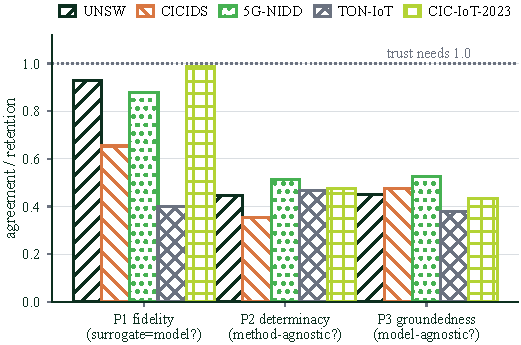
\includegraphics[width=0.92\columnwidth]{fig_trust.pdf}
\caption{Each necessary property, measured on three modern NIDS datasets. A sound trust signal
requires every bar at $1.0$; all fall short on every dataset.}
\label{fig:trust}
\end{figure}

\textbf{Fidelity fails (Property~\ref{p:fid}).} We take a KAN-IDS, whose per-edge functions are
its interpretability selling point, and extract the interpretable form its proponents invoke, a
low-order symbolic surrogate of each edge. Detection $F_1$ drops by
$0.074{\pm}0.021$ on UNSW-NB15,
$0.321{\pm}0.079$ on CICIDS2017, and
$0.116{\pm}0.01$ on 5G-NIDD. On CICIDS2017 the
interpretable form collapses from $F_1=0.889$ to
$0.541$ (Fig.~\ref{fig:fidelity}): the readable model is nearly a
different, and far worse, detector. A post-hoc check agrees: keeping only the top-5 attributed
features reproduces the 5G-NIDD detector's decision on just $0.631$ of flows,
so the reason does not even suffice for the decision. The analyst reasons about a model that is
not the one guarding the network.

\begin{figure}[t]
\centering
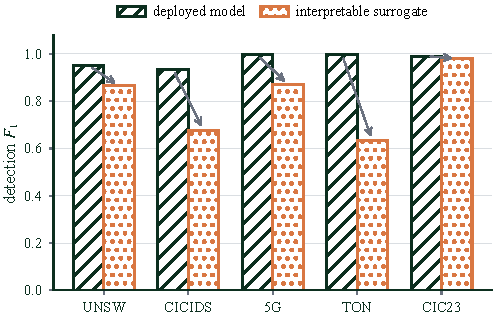
\includegraphics[width=0.82\columnwidth]{fig_fidelity.pdf}
\caption{Fidelity fails. The interpretable surrogate of a KAN-IDS detects markedly worse than the
deployed model, collapsing on CICIDS2017. The analyst reasons about the lower bar.}
\label{fig:fidelity}
\end{figure}

\textbf{Determinacy fails (Property~\ref{p:det}).} For the same detector and the same
flagged-malicious flows, we measure how much the top-5 features agree across explainers. Among
the three gradient-family methods, mean agreement is only
$0.454{\pm}0.017$ (UNSW-NB15),
$0.361{\pm}0.005$ (CICIDS2017), and
$0.526{\pm}0.079$ (5G-NIDD). Crucially, this is not
an artifact of using only gradient methods: adding the two most deployed model-agnostic
explainers, SHAP and LIME, drives agreement lower still (Table~\ref{tab:breadth}), and \emph{SHAP
and LIME agree with each other on only} $0.258$--$0.251$
\emph{of the top-5 features they show}. The reason presented to the analyst is largely an artifact
of which equally-defensible tool the vendor shipped.

\begin{table}[t]
\centering
\caption{Determinacy across five explainers: mean top-5 agreement over all pairs, and the
agreement of SHAP with LIME, the two most deployed model-agnostic explainers. Even these two
disagree on roughly four of every five features shown.}
\label{tab:breadth}
\small\setlength{\tabcolsep}{3.5pt}
\begin{tabular}{lccc}
\toprule
& UNSW-NB15 & CICIDS2017 & 5G-NIDD \\
\midrule
mean, all 5 explainers & $0.329$ & $0.286$ & $0.50$ \\
SHAP vs.\ LIME        & $0.258$ & $0.207$ & $0.251$ \\
gradient vs.\ SHAP    & --- & $0.147$ & --- \\
\bottomrule
\end{tabular}
\end{table}

\textbf{Groundedness fails (Property~\ref{p:grnd}).} We train four detectors that differ only in
random seed. Their detection performance is statistically identical (on UNSW-NB15,
$F_1=0.953{\pm}0.001$), yet their top-5 explanations
for the same inputs agree on only
$0.533{\pm}0.005$ (UNSW-NB15),
$0.618{\pm}0.029$ (CICIDS2017), and
$0.555{\pm}0.027$ (5G-NIDD) of features. An analyst
handed one detector's explanation is trusting an accident of training that an equally good
detector would contradict.

All three necessary properties fail, with tight seed-to-seed variance, across three modern
datasets. The trust that explainable ML-IDS invites is therefore, as currently produced, not
well-founded.

% ============================================================================
\section{Can an Adversary Exploit This?}\label{sec:adv}
% ============================================================================
The failures above are benign: they arise without an adversary. Security demands the adversarial
case. If an attacker can craft a malicious flow that the detector still flags but whose
explanation points at innocuous features, the analyst may dismiss a true alarm, an evasion by
explanation rather than by detection. In vision and NLP this is established: explanations can be
moved almost arbitrarily while the prediction is fixed~\cite{ghorbani2019,dombrowski2019,slack2020}.

We tested the analogue on our tabular IDS. We model an analyst who reasons from explanations as an
auditor classifier trained to map an attribution vector to benign/attack, and we search for a
bounded perturbation that keeps the detector's malicious decision while steering the explanation
toward the benign prototype. Honestly, the attack was inconclusive: the detector kept firing on
$1.0$ of flows, but the manipulated explanations were still read as
attack by the auditor almost everywhere, and the fraction of true alarms we could get dismissed
never exceeded $0.260$, most of which reflects the auditor's baseline
error rather than the attack. A second formulation, directly driving attribution mass off the
top-$k$ features, also failed to move them.

We do not claim tabular IDS explanations are robust. We think the gap from the vision result is
real and informative: tabular NIDS features are low-dimensional and semantically constrained, so
the room to reshape an explanation without either flipping the decision or leaving the data
manifold is small, unlike the high-dimensional redundancy of images. Stronger, model-agnostic
attacks in the style of adversarial scaffolding~\cite{slack2020} remain untested here and are a
clear next step. We report the negative result because a security paper should not overstate an
attack, and because the benign failures of Section~\ref{sec:fail} already void trust without
needing an adversary.

% ============================================================================
\section{A Reliability Gate for Explanations}\label{sec:defense}
% ============================================================================
If interpretability-based trust fails by default, the constructive question is whether we can
tell the analyst \emph{when} an explanation may be trusted, rather than asking for blind trust or
none. We propose a per-alarm \emph{reliability gate}.

\textbf{What ``reliable'' means.} We call an explanation reliable for a flow if it is
\emph{stable}: its top-$k$ features are reproduced both across an ensemble
$\{f_1,\dots,f_E\}$ of equally-good models (groundedness holds locally) and across the attribution
family $\mathcal{M}$ (determinacy holds locally). We combine the two into a per-flow reliability
score, where $\bar{J}$ denotes the mean pairwise top-$k$ agreement over the indicated set,
\begin{equation}
S(x)=\tfrac{1}{2}\,\bar{J}_{\text{model}}(x)\;+\;\tfrac{1}{2}\,\bar{J}_{\text{method}}(x),
\label{eq:stab}
\end{equation}
with $\bar{J}_{\text{model}}$ taken over the ensemble $\{f_i\}$ (local groundedness, P3) and
$\bar{J}_{\text{method}}$ over the family $\mathcal{M}$ (local determinacy, P2).
$S(x)$ is the ground truth we want but cannot compute per alarm in deployment, since it needs an
ensemble and several explainers. We stress that $S$ measures \emph{stability, not correctness}: a
stable explanation is reproducible, not necessarily faithful, so the gate below recovers a
necessary component of trust, not all of it (Section~\ref{sec:disc}).

\textbf{The gate.} We train a lightweight detector to predict this stability from signals that a
single deployed model exposes at alarm time: the decision margin, the concentration (entropy) of
the attribution, a local linear-surrogate fidelity, and an out-of-distribution distance. If the
cheap detector predicts the expensive stability well, the analyst can be told, for free, when not
to trust an explanation.

\textbf{It works.} Across datasets the gate predicts explanation reliability with AUC
$0.722{\pm}0.023$ (UNSW-NB15),
$0.852{\pm}0.002$ (CICIDS2017), and
$0.944{\pm}0.000$ (5G-NIDD) over three seeds
(Fig.~\ref{fig:defense}). Gating on it separates reliable from unreliable explanations: on
5G-NIDD the flows the gate passes are $0.272$ more stable, in
absolute terms, than those it flags.

\textbf{It is not just an OOD detector.} A natural worry is that the gate merely detects
out-of-distribution flows, for which everything is uncertain. It does not. Ablating to each
single signal (Table~\ref{tab:defense}), the out-of-distribution distance alone reaches only AUC
$0.477$ on CICIDS2017, below chance, while the full gate reaches
$0.850$; there, the explanation-specific concentration signal
($0.713$) carries the prediction. On every dataset the full gate beats
every single-signal baseline, so its power is not reducible to confidence or distribution
distance. This is a first, deliberately simple mechanism; richer stability predictors are an
obvious extension.

\begin{figure}[t]
\centering
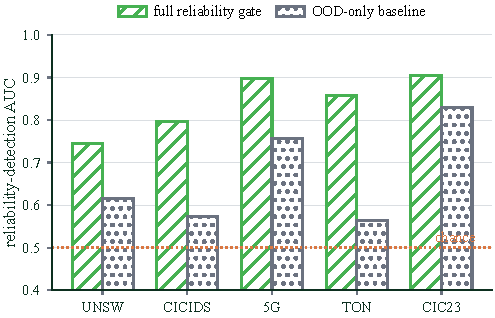
\includegraphics[width=0.82\columnwidth]{fig_defense.pdf}
\caption{The reliability gate predicts, per alarm and from one model, whether an explanation is
trustworthy (high AUC), and is not reducible to an out-of-distribution detector, which alone is
near or below chance on CICIDS2017.}
\label{fig:defense}
\end{figure}

\begin{table}[t]
\centering
\caption{Reliability-gate AUC: the full detector versus each single signal. The full gate beats
every single signal on every dataset; out-of-distribution distance alone is weak or useless,
ruling out the ``it is just OOD'' explanation.}
\label{tab:defense}
\small\setlength{\tabcolsep}{3.5pt}
\begin{tabular}{lccc}
\toprule
& UNSW-NB15 & CICIDS2017 & 5G-NIDD \\
\midrule
full gate       & $\mathbf{0.73}$ & $\mathbf{0.85}$ & $\mathbf{0.94}$ \\
margin only     & $0.61$ & $0.43$ & $0.67$ \\
concentration only & $0.63$ & $0.71$ & $0.92$ \\
local fidelity only & $0.63$ & $0.60$ & $0.66$ \\
OOD distance only  & $0.70$ & $0.48$ & $0.85$ \\
\bottomrule
\end{tabular}
\end{table}

% ============================================================================
\section{Threat-Aware Evaluation Criteria}\label{sec:criteria}
% ============================================================================
If interpretability is to warrant trust in a security setting, a claim to that effect should be
held to checkable conditions. We propose the following, each the operational counterpart of a
property or result above, and each currently unmet by typical explainable-IDS papers.

\begin{enumerate}
\item \textbf{Fidelity budget.} Report the decision agreement between the interpretable artifact
the analyst sees and the deployed model, on held-out and on attack traffic. A trust claim below a
stated threshold is unsupported.
\item \textbf{Method invariance.} Report top-feature agreement across at least two standard
attribution methods, including a perturbation-based one (SHAP or LIME). If the shown reason
changes with the method, disclose it; do not present one method's output as \emph{the}
explanation.
\item \textbf{Instance invariance.} Report explanation agreement across performance-equivalent
retrainings. Explanations that vary across equally-good models must not be sold as task insight.
\item \textbf{Adversarial robustness of the explanation.} State a threat model for the
explanation itself and evaluate whether an adversary preserving the malicious decision can alter
the shown reason. Absent this, interpretability is a usability feature, not a security one.
\item \textbf{Trust as warrant, not satisfaction.} Evaluate whether acting on the explanation
agrees with ground truth, not whether analysts \emph{feel} more confident.
\item \textbf{Reliability signalling.} Where per-flow reliability varies, provide a gate that
tells the analyst when the explanation should not be trusted, and validate it.
\end{enumerate}

These are necessary, not sufficient; but a claim that fails any of them should not be stated as a
security benefit. They are cheap to run; we release code that computes all six.

% ============================================================================
\section{Discussion}\label{sec:disc}
% ============================================================================
\textbf{Accountability.} Operational security increasingly places explanations in the decision
loop and, implicitly, in the accountability chain: an analyst who acts ``because the system
showed feature $X$'' is relying on $e$. Our results imply this reliance is, today, reliance on an
artifact of tool and seed. Accountability regimes that credit ``the model is explainable'' as a
control are mis-specified unless the explanation meets conditions like ours, and the reliability
gate is a step toward making the credit conditional on evidence.

\textbf{Why a gate rather than a fix.} We do not claim to make explanations faithful,
determinate, and grounded; that may be impossible for post-hoc attributions on expressive models.
The gate is more modest and more deployable: it accepts that reliability varies per flow and
surfaces it, so trust can be selective. This mirrors how mature security tooling treats
uncertain signals, by scoring confidence rather than asserting it.

\textbf{Scope and honesty.} Our demonstrations use gradient- and perturbation-family attributions
and one symbolic-surrogate notion of interpretability; prototype- and rule-based methods may
behave differently, and testing them is what our criteria call for. Our adversarial result is
deliberately reported as inconclusive. The reliability gate is a first mechanism with a modest
AUC on one dataset ($0.72$ on UNSW-NB15); we expect better stability predictors to improve it.
The point is not that these particular methods are uniquely bad, but that the \emph{inference}
from interpretability to trust is unlicensed until the properties are checked, and on modern data
the check fails by default.

% ============================================================================
\section{Ethics Considerations}\label{sec:ethics}
% ============================================================================
This work studies public network-intrusion datasets (UNSW-NB15, CICIDS2017, 5G-NIDD) and
introduces no new data collection or human-subjects experiment; the analyst in our study is
modeled by a classifier, not a person, so no IRB approval was required. The paper is a defensive
contribution: it warns that a widely promoted security workflow, trusting ML-IDS through
explanations, may be unfounded, and offers a mechanism to mitigate the risk. Our inconclusive
attack is described at a level sufficient to reproduce the analysis but does not provide an
operational tool for evading detectors, and the underlying benign failures are the primary basis
of our conclusions. We will release code and evaluation criteria to help the community audit
interpretability-for-trust claims, which we judge net-beneficial: the same code that could reveal
a weak explanation is what a defender needs to avoid over-trusting one. We disclose no specific
vulnerable product; the concern is a methodological one affecting the class of explainable ML-IDS.

% ============================================================================
\section{Conclusion}\label{sec:concl}
% ============================================================================
Explainable ML-IDS invites analysts to trust detectors through their explanations. We asked what
would make that trust well-founded, formalized it as fidelity, determinacy, and groundedness, and
showed all three fail on three modern intrusion datasets and across five standard explainers,
including SHAP and LIME. We found the failure hard to weaponize on tabular IDS, an honest negative
result, but easy to demonstrate benignly. We then turned the diagnosis into a defense, a per-alarm
reliability gate that predicts when an explanation may be trusted with AUC up to $0.94$ and is not
reducible to out-of-distribution detection. Interpretability, as currently produced and evaluated,
is not a sound basis for trust in ML-IDS; but the conditions under which it would be are checkable,
and reliability is partly recoverable. We hope the criteria and the gate move explainable
intrusion detection from measuring the trust it induces to earning the trust it deserves.

\bibliographystyle{IEEEtran}
\bibliography{refs}
\end{document}
